\section{Sensitivity and convergence of MULTI}
\label{sec:ablation}

\subsection{The threshold $\epsilon$}
We ran MULTI for 21 log-spaced values $\epsilon\in[10^{-5},10^{-1}]$ on all 24 problems
(Fig.~\ref{fig:eps}).
\begin{itemize}[leftmargin=*,itemsep=1pt]
\item \textbf{Flat optimum, steep cliff.} RE$(\epsilon)$ is nearly flat over
  1--2 decades below the optimum and then rises steeply. Choosing $\epsilon$
  too \emph{small} is cheap: $\lambda$ becomes unbounded in flat regions, but the
  data term and the curvature term still balance. Choosing it too \emph{large}
  is expensive: $\lambda_i\approx\|A\mathbf u-\mathbf b\|^2/(N\epsilon)$ becomes small and
  uniform, so noise is under-regularised everywhere.
\item \textbf{The best $\epsilon$ is set by the image, not by the noise.} Within one
  image the oracle $\epsilon$ hardly changes with $\delta$ (right panel; points of one
  colour lie on a near-horizontal band). Across images it spans three
  decades: about $10^{-4}$ for ct\_head, about $3\times10^{-3}$ for cat/portrait and
  about $6\times10^{-2}$ for satellite. As a result, the ratio $\epsilon_{\rm opt}/\hat\sigma^2$
  ranges from \nRatioLo{} to \nRatioHi{} for the natural and medical images, and from
  \nRatioSatLo{} to \nRatioSatHi{} for satellite.
  This contradicts the natural guess $\epsilon\propto\sigma^2$, which we had used
  for our first automatic rule. The explanation is that $\epsilon$ is compared with $S_i$,
  the \emph{restored} curvature, which reflects the image content much more
  than the noise.
\end{itemize}

\begin{figure}[t]
\centering
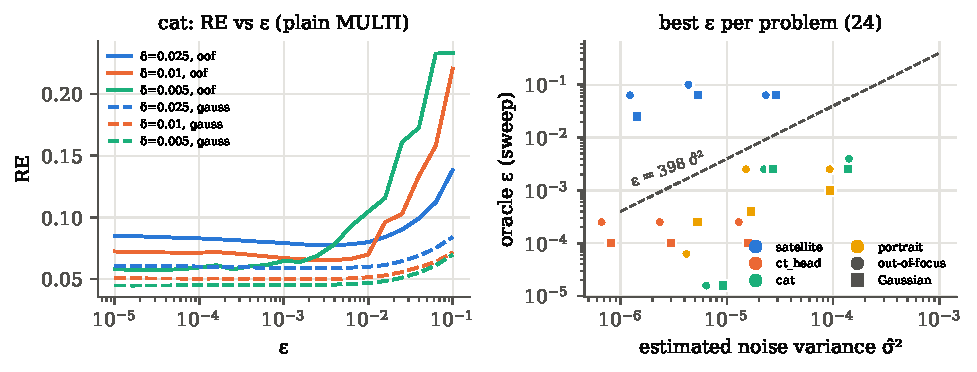
\includegraphics[width=0.85\linewidth]{figures/eps_sweep.pdf}
\caption{Left: RE vs.\ $\epsilon$ for cat (solid: out-of-focus, dashed: Gaussian).
Right: the best $\epsilon$ of every problem against the estimated noise variance.
The best $\epsilon$ clusters by image, not along the line $\epsilon\propto\hat\sigma^2$.}
\label{fig:eps}
\end{figure}

\subsection{The neighbourhood size $R$}
For every $R\in\{1,3,5,9,15\}$ we re-tuned $\epsilon$ ($\delta=10^{-2}$, both blurs,
Fig.~\ref{fig:R}). The best $R$ is 3 or 5 for every problem. $R=1$, i.e.\ no max filter,
is clearly worse (on average $+\nRoneLoss\%$ RE relative to the best $R$, up to
$+\nRoneLossMax\%$ on ct\_head). The Laplacian of an edge changes sign
exactly at the edge, so without the max filter $\lambda_i$ is \emph{large} on the edge
itself and the edge gets smoothed. Large windows hurt too, though less
($R=15$: $+\nRfifteenLoss\%$ on average, up to $+\nRfifteenLossMax\%$): the low-$\lambda$ zone
around every edge widens, so noise survives next to edges. The paper's default $R=5$ is on
average within \nRfiveLoss\% of the best $R$ (at worst \nRfiveLossMax\%). Satellite prefers
$R=3$, which agrees with the paper's choice of $R=3$ for its galaxy image; ct\_head, with its
thin bone and soft-tissue contours, is the most sensitive to $R$ in both directions.

\begin{figure}[t]
\centering
\begin{minipage}[t]{0.49\linewidth}\vspace{0pt}
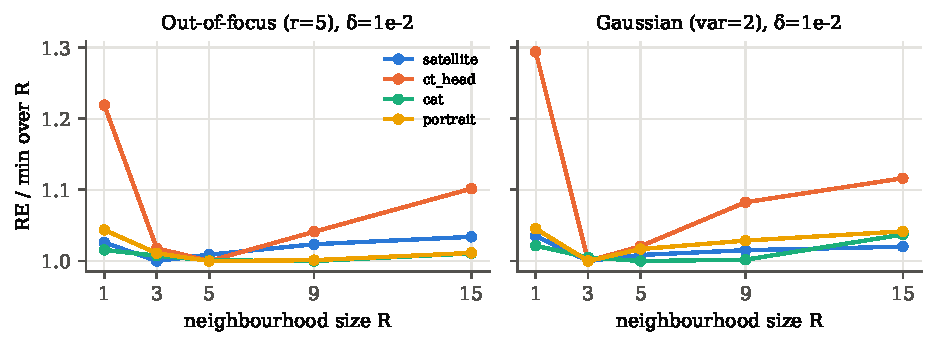
\includegraphics[width=\linewidth]{figures/R_sweep.pdf}
\caption{RE (relative to the best $R$) vs.\ neighbourhood size; $\epsilon$ re-tuned for each $R$.}
\label{fig:R}
\end{minipage}\hfill
\begin{minipage}[t]{0.49\linewidth}\vspace{0pt}
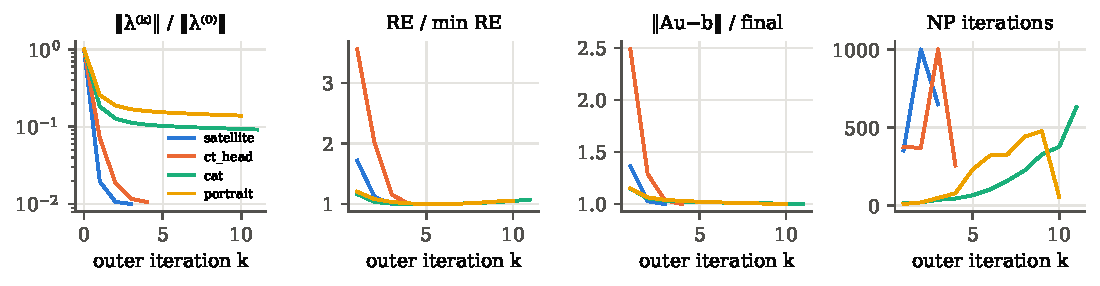
\includegraphics[width=\linewidth]{figures/convergence.pdf}
\caption{Algorithm~1 histories (out-of-focus, $\delta=10^{-2}$, oracle $\epsilon$, $\mathrm{Tol}=0$).}
\label{fig:conv}
\end{minipage}
\end{figure}

\subsection{Convergence of Algorithm~1}
With $\mathrm{Tol}=0$ (Fig.~\ref{fig:conv}), as in the paper's Figure~10, $\|\boldsymbol\lambda\|$
drops by one to two orders of magnitude in the first 2--4 outer iterations and then
settles. RE reaches its minimum after 3--5 outer iterations, and the residual
stabilises at the same time. The cost of an outer iteration grows as $\boldsymbol\lambda$
becomes more heterogeneous, because the BCCB preconditioner, built from the
\emph{mean} $\lambda$, then fits the true Hessian less well, so NP needs more iterations. The
paper's $\mathrm{Tol}=10^{-1}$ stops after 3--5 outer iterations, close to the RE
minimum. Note, however, that RE starts to \emph{rise} again for cat and portrait. This
leads to the failure mode in the next section.

\section{Extension 1: $\lambda$-collapse and a noise-floor safeguard}
\label{sec:collapse}
Our first automatic variant (Sec.~\ref{sec:auto}) failed catastrophically on two
problems, cat and portrait under out-of-focus blur at $\delta=0.5\%$, where it gave
\emph{negative} ISNR ($-1.6$\,dB, worse than the blurred input). The iteration
histories (Fig.~\ref{fig:collapse}) reveal a positive feedback loop in
Algorithm~1:
\begin{center}
residual $\|A\mathbf u-\mathbf b\|$ below the noise level
$\Rightarrow$ $\lambda_i\propto\|A\mathbf u-\mathbf b\|^2$ shrinks
$\Rightarrow$ the next solve fits more noise
$\Rightarrow$ the residual drops further $\Rightarrow\dots$
\end{center}
The numerator of $\lambda_i$ is the current residual, which is an estimate of the noise
energy $N\sigma^2$. Once the solution starts to over-fit, this estimate becomes
\emph{biased low}, and nothing in the rule pulls it back up. $\|\boldsymbol\lambda\|$ then
decays geometrically, so the $\lambda$-change test ($\mathrm{Tol}$) never fires
and the iteration runs for all 20 outer iterations. On cat, RE falls to
\nCollReMin{} at outer iteration \nCollKmin{} and then climbs back to \nCollReFinal.
This is the classical \emph{semi-convergence} of iterative regularisation~\cite{engl},
appearing here in a fixed-point method that is supposed to be ``automatic''.
It occurs when $\epsilon$ is large relative to the curvature scale and the noise is low.
In the paper's oracle setting, a too-large $\epsilon$ is simply never selected, which is
probably why the paper does not report it.

\paragraph{Fix, first attempt: discrepancy stop.} The residual should never fall
below the noise level. Our first fix stops Algorithm~1 as soon as
$\|A\mathbf u^{(k)}-\mathbf b\|\le\tau\sqrt N\,\hat\sigma$ ($\tau=1$), which is Morozov's
discrepancy principle~\cite{morozov}. Here $\hat\sigma$ is the robust MAD noise estimate
from the finest diagonal Haar wavelet coefficients,
$\hat\sigma=\mathrm{median}|HH|/0.6745$~\cite{donoho}, so no ground truth is needed.
This removes the catastrophic failures (stars in Fig.~\ref{fig:collapse}), but the dense
$\epsilon$-sweep shows that it stops \emph{too early}: usually after 1--2 outer
iterations, before $\boldsymbol\lambda$ has adapted to the image. Its best RE is on average
\nStopMinLoss\% worse than that of the plain algorithm.

\paragraph{Fix, final: a noise floor in the $\lambda$ rule.} The root cause is that
the numerator of $\lambda_i$ can drop below the true noise energy. We therefore floor it:
\begin{equation}
\lambda_i=\frac{\max\big(\|A\mathbf u-\mathbf b\|^2,\ N\hat\sigma^2\big)}{N\,(S_i+\epsilon)} .
\label{eq:floor}
\end{equation}
While the residual is above the noise level, this is exactly the paper's rule. When the
residual would fall below it, the overall scale of $\boldsymbol\lambda$ is frozen at the
discrepancy level, but the iteration continues to refine \emph{where} the smoothing goes
(through $S_i$). The positive feedback loop is broken, and the usual $\mathrm{Tol}$ test
then terminates the iteration. The cost is one scalar $\max$ per outer iteration.
Over the sweep (Fig.~\ref{fig:epssafe}), the floored algorithm's best RE differs from that of
the plain algorithm by \nFloorMinLoss\% on average (equal or better on \nFloorBetter/24
problems), so nothing is lost when no collapse occurs. It is also less sensitive to
$\epsilon$: the median ratio of worst to best RE over the four decades of $\epsilon$ drops
from \nWorstPlain{} (plain) to \nWorstFloor{}. This sweep caps every run at 2000 NP
iterations, which cuts the collapse short and therefore \emph{understates} the benefit.
With the full budget used by MULTI-auto (Table~\ref{tab:variants}), the floor raises the
worst-case ISNR from \nVarNoneWorst\,dB (no safeguard) and \nVarStopWorst\,dB (discrepancy
stop) to \nVarFloorWorst\,dB, and gives the best mean ISNR (\nVarFloorMean\,dB) and the
smallest average loss to the oracle (\nVarFloorLoss\,dB). The plain rule is within
0.5\,dB of the oracle slightly more often (\nVarNoneWithin{} vs.\ \nVarFloorWithin{} of 24),
but it fails badly on the problems where it collapses.

\begin{table}[t]
\centering\small
\inputtable{tables/auto_variants.tex}
\caption{MULTI-auto on the 24 main problems with each $\lambda$-collapse safeguard
($\kappa$ re-calibrated for each variant on its own $\epsilon$-sweep, except ``none'', which
uses our initial calibration). ISNR and MSSIM are means; ``worst'' is the worst single
problem; ``loss'' is the mean ISNR gap to oracle-tuned MULTI, and the last column counts the
problems within 0.5\,dB of it. The last row is MULTI-autoS (Sec.~\ref{sec:auto}).}
\label{tab:variants}
\end{table}

\begin{figure}[t]
\centering
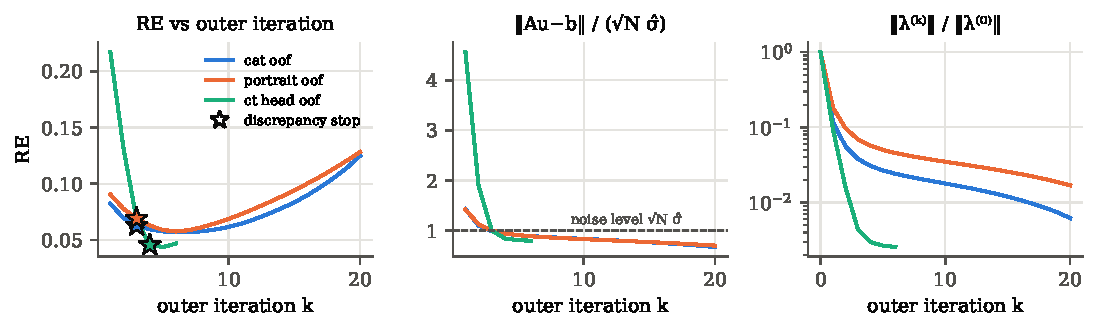
\includegraphics[width=\linewidth]{figures/lambda_collapse.pdf}
\caption{$\lambda$-collapse of MULTI with automatic $\epsilon$ and no safeguard
(out-of-focus, $\delta=0.5\%$). Once the residual crosses the noise level (dashed),
$\|\boldsymbol\lambda\|$ keeps decaying and RE grows. Stars: where the discrepancy
stop (our first fix) would end the iteration.}
\label{fig:collapse}
\end{figure}

\section{Extension 2: fully automatic MULTI (MULTI-auto)}
\label{sec:auto}
The paper chooses $\epsilon$ by minimising RE against the ground truth, which is not
possible in real use. MULTI-auto sets
\[
\epsilon=\kappa\,\hat\sigma^2,\qquad \text{with the noise-floor rule~\eqref{eq:floor}},
\]
with one global constant $\kappa$, calibrated once on the 24 main problems and then
\emph{frozen}. The calibration minimises the mean relative RE loss with respect to the
per-problem oracle $\epsilon$, read off the noise-floor sweep (Fig.~\ref{fig:epssafe}, right);
it gives $\kappa=\nKappa$. The rationale is dimensional: $\epsilon$ is a curvature
threshold, and the variance of the discrete Laplacian of pure noise is $20\sigma^2$.
Note that this rule is at odds with our sweep, where the best $\epsilon$ barely grows with
$\sigma$ (Sec.~\ref{sec:ablation}); we return to this below.

\paragraph{Results on the main set.} With no tuning at all, MULTI-auto is on average
\nMainAutoLoss\,dB (median \nMainAutoLossMedian\,dB) below oracle-tuned MULTI,
and within 0.5\,dB of it on \nMainAutoWithinHalf/\nMainN{} problems. It beats
oracle-tuned TIKH on \nMainAutoBeatsTikh, oracle TV on \nMainAutoBeatsTV{} and oracle
TGV on \nMainAutoBeatsTGV{} of the \nMainN{} problems. Each oracle baseline needed
10--20 runs \emph{and the ground truth} to choose its parameter. In RE terms the average
loss is \nMainAutoRelLoss\%, but the worst problem loses \nMainAutoRelLossMax\%. The large
losses are all at $\delta=2.5\%$, where $\kappa\hat\sigma^2$ overshoots the best
$\epsilon$ by about an order of magnitude. Since $\lambda_i\propto 1/(S_i+\epsilon)$, the weights
then become roughly $15\times$ too small and almost uniform: MULTI under-regularises, leaves
noise in flat regions and loses most of its adaptivity.

\begin{figure}[t]
\centering
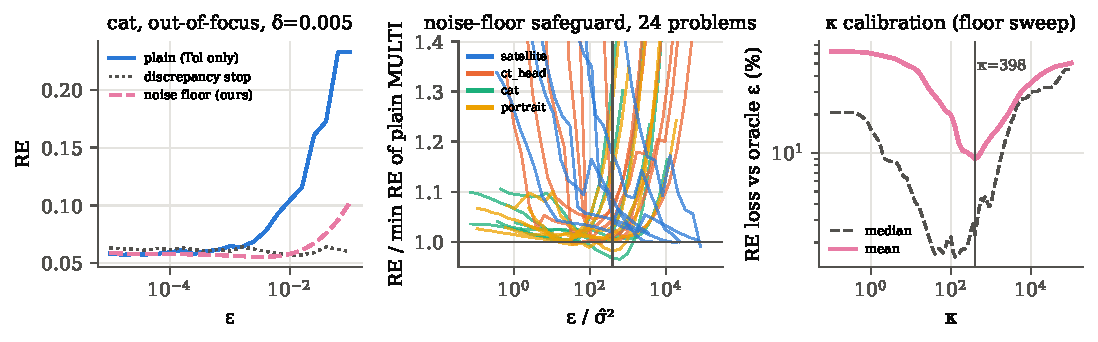
\includegraphics[width=\linewidth]{figures/eps_safe.pdf}
\caption{Left: RE vs.\ $\epsilon$ on the collapse case for plain MULTI and both safeguards.
Middle: noise-floor RE$(\epsilon)$ for all 24 problems, relative to the best RE of plain MULTI.
Right: calibration of $\kappa$ (mean and median relative RE loss over the 24 problems).}
\label{fig:epssafe}
\end{figure}

\paragraph{A scale-aware alternative.} Since the best $\epsilon$ follows the image's
curvature scale (Sec.~\ref{sec:ablation}), we also tried
$\epsilon=c\cdot Q_q\big(S(\mathbf u_{\rm pilot})\big)$, a quantile of the local curvature
of a cheap pilot restoration. The pilot is Laplacian-Tikhonov with $\lambda$ set by the
discrepancy principle, solved in closed form by FFT, which costs about 40 FFT solves.
We evaluated it against the $\kappa\hat\sigma^2$ rule with \emph{leave-one-image-out}
calibration: the constant is fitted on three images and tested on the
fourth. With $\epsilon$ read off the sweep curves, the best quantile ($q=\nScaleBest$, $c\approx\nScaleC$
when fitted on all four images) gives a mean held-out RE loss of \nLoioBestMean\% with respect
to the per-problem oracle $\epsilon$ (median \nLoioBestMedian\%, worst \nLoioBestMax\%). The
$\kappa\hat\sigma^2$ rule, evaluated the same way, gives \nLoioSigMean\% (median
\nLoioSigMedian\%, worst \nLoioSigMax\%). Per held-out image, the scale-aware rule loses
\nLoioBestCat\% (cat), \nLoioBestPortrait\% (portrait), \nLoioBestCthead\% (ct\_head) and
\nLoioBestSatellite\% (satellite), against \nLoioSigCat\%, \nLoioSigPortrait\%,
\nLoioSigCthead\% and \nLoioSigSatellite\% for $\kappa\hat\sigma^2$. Satellite is the hardest
case for both rules: its best $\epsilon$ lies at the upper end of the sweep grid, and at small
$\epsilon$ many of its sweep runs hit the NP budget, so its curves are the least reliable.

\paragraph{Full runs: MULTI-autoS.} The sweep curves are only a proxy (2000-NP cap), so we also
ran the rule for real. MULTI-autoS uses $\epsilon=c\,Q_{\nScaleBest}(S(\mathbf u_{\rm pilot}))$
with $c=\nScaleC$, the noise floor and the full budget; nothing else changes. On the main set
(where $c$ is in-sample) it is on average \nMainAutoSLoss\,dB below oracle MULTI, against
\nMainAutoLoss\,dB for MULTI-auto; it is within 0.5\,dB of the oracle on
\nMainAutoSWithinHalf/\nMainN{} problems (MULTI-auto: \nMainAutoWithinHalf), and its worst RE
loss drops from \nMainAutoRelLossMax\% to \nMainAutoSRelLossMax\%
(Table~\ref{tab:variants}, last row). The gain is concentrated at $\delta=2.5\%$, exactly where
$\kappa\hat\sigma^2$ overshoots.

For a held-out test we ran both automatic rules on the 12 Kodak images at the two noise levels
where they differ (no oracle needed). At $\delta=2.5\%$, MULTI-autoS is better on
\nKRHiWins/\nKRHiN{} problems, by \nKRHiGain\,dB ISNR on average (up to \nKRHiBestGain\,dB;
mean RE change \nKRHiRelRE\%). At $\delta=0.5\%$ the two rules are level
(\nKRLoGain\,dB on average, better on \nKRLoWins/\nKRLoN{}, worst \nKRLoWorstGain\,dB), and at
$\delta=1\%$, where $\kappa$ is effectively calibrated, they are also level
(\nISNRKodakAutoS{} vs.\ \nISNRKodakAuto\,dB, Table~\ref{tab:kodak}). So the scale-aware rule
removes the high-noise failure of $\kappa\hat\sigma^2$ with no systematic loss elsewhere, at the cost of
one pilot solve (about 40 FFTs). We keep $\kappa\hat\sigma^2$ as ``MULTI-auto'' in the main
tables because it was fixed before these experiments; MULTI-autoS is reported alongside it.



\section{Extension 3: generalisation to unseen Kodak images}
\label{sec:kodak}
To check that the conclusions are not specific to four hand-picked images, we
repeated the comparison on 12 Kodak images that were not used for any design
decision (Fig.~\ref{fig:kodak}). There are \nKodakN{} problems: both blurs at $\delta=1\%$.
TIKH, TV, TGV and MULTI are again oracle-tuned per problem, while MULTI-auto uses the
\emph{frozen} $\kappa=\nKappa$.

\begin{figure}[t]
\centering
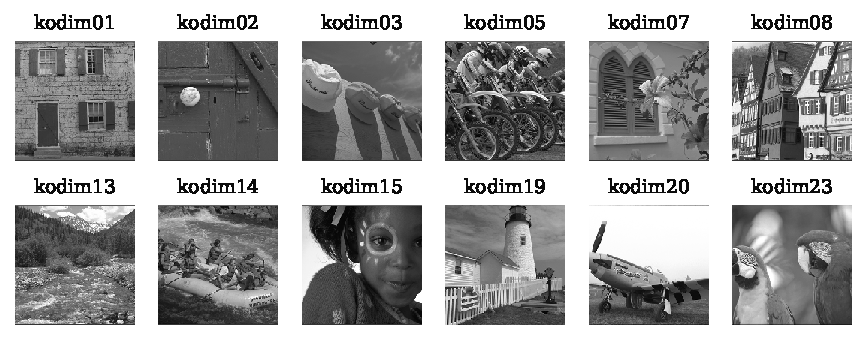
\includegraphics[width=0.9\linewidth]{figures/kodak_images.pdf}
\caption{The 12 Kodak generalisation images (grayscale, $256^2$).}
\label{fig:kodak}
\end{figure}

\begin{figure}[t]
\centering
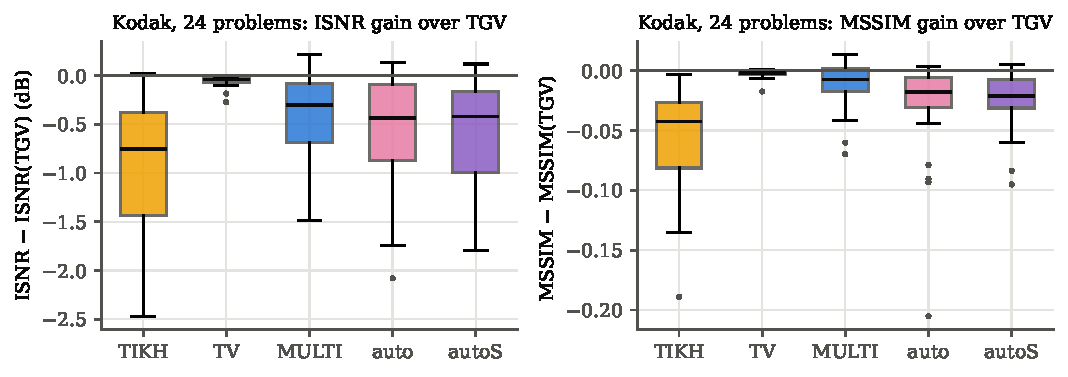
\includegraphics[width=0.9\linewidth]{figures/kodak_gain.pdf}
\caption{Kodak: per-problem ISNR and MSSIM difference with respect to oracle TGV.}
\label{fig:kodakgain}
\end{figure}

\begin{table}[t]
\centering\small
\inputtable{tables/kodak_isnr.tex}
\caption{Kodak: mean ISNR (dB) per blur.}
\label{tab:kodak}
\end{table}

The blur dependence carries over, but in a milder form (Fig.~\ref{fig:kodakgain},
Table~\ref{tab:kodak}). Under Gaussian blur, MULTI and TGV are close: MULTI is on average
\nKodakGainTGVGauss\,dB from TGV and is the best tuned method on \nKodakWinsGauss/\nKodakNGauss{}
images. Under out-of-focus blur TGV is clearly ahead (\nKodakGainTGVOof\,dB; MULTI best on
\nKodakWinsOof/\nKodakNOof). So MULTI's Gaussian-blur advantage on the main set does not
generalise to these small, texture-rich photographs, where TGV's sparsity prior pays off.
MULTI still beats TIKH, which uses the same penalty, on \nKodakMultiBeatsTikh/\nKodakN{}
problems (by \nKodakMultiTikhGain\,dB on average). MULTI-auto, which never saw these images, is
on average only \nKodakAutoLoss\,dB below oracle MULTI and within 0.5\,dB of it on
\nKodakAutoWithinHalf/\nKodakN{} problems.

\section{Extension 4: colour images}
\label{sec:color}
MULTI extends to RGB with no change to the model: we run MULTI-auto independently on
each channel, each with its own $\hat\sigma$, $\epsilon$ and $\boldsymbol\lambda$ map. As a baseline,
we run channel-wise TGV with a single $\lambda$ that is oracle-tuned on the colour RE.
On \texttt{kodim23} (parrots) and \texttt{kodim05} (motorbikes) with out-of-focus blur
at $\delta=1\%$ (Fig.~\ref{fig:color}), MULTI-auto reaches
\nColParrotsAutoPSNR\,dB / SSIM \nColParrotsAutoSSIM{} and
\nColBikesAutoPSNR\,dB / \nColBikesAutoSSIM{}, against
\nColParrotsTGVPSNR\,dB / \nColParrotsTGVSSIM{} and \nColBikesTGVPSNR\,dB / \nColBikesTGVSSIM{}
for oracle TGV (blurred input: \nColParrotsBlurPSNR{} and \nColBikesBlurPSNR\,dB).
Without any tuning, MULTI-auto gains 4.4--5.5\,dB over the blurred input and stays within
1\,dB of ground-truth-tuned TGV, in line with the grayscale out-of-focus results. Its SSIM
deficit on the parrots comes from the smooth, defocused background: the three channels get
independent $\boldsymbol\lambda$ maps, so noise that survives in one channel but not in the
others appears as coloured speckle, which the eye (and SSIM) notices more than grey noise.
A natural improvement is a single curvature map $S_i$, computed from the luminance (or as
$\max_c S_i^{(c)}$) and shared by all channels.

\begin{figure}[t]
\centering
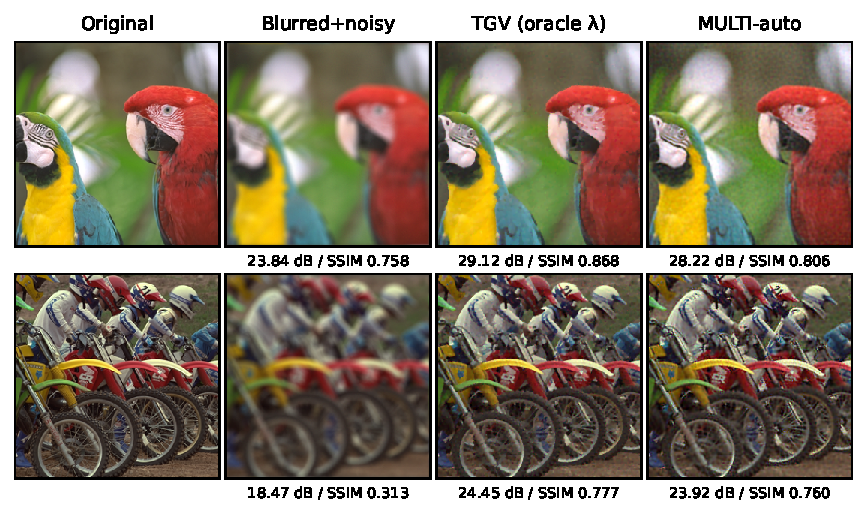
\includegraphics[width=0.9\linewidth]{figures/color.pdf}
\caption{Colour restoration (out-of-focus, $\delta=1\%$), channel-wise. Below each image: PSNR / SSIM.}
\label{fig:color}
\end{figure}
